%
% chapter.tex -- Orientierung und Vektorprodukt
%
% (c) 2018 Prof Dr Andreas Müller, Hochschule Rapperswil
%
\chapter{Orientierung und Vektorprodukt\label{chapter:orientierung}}
\lhead{Orientierung und Vektorprodukt}
\rhead{}
Die Determinante von Kapitel~\ref{chapter-determinanten} hat noch
keine geometrische Anwendung.
In diesem Kapitel soll gezeigt werden, wie die Determinante ermöglich,
den geometrischen Raum zu orientieren.
In der Ebene heisst das, zwischen Uhrzeigersinn und Gegenurzeigersinn
unterscheiden zu können, im dreidimensionalen Raum geht es um die
Unterscheidung zwischen rechts und links.
Als Nebenprodukt erhalten wir für den dreidimensionalen Raum das
besonders handliche Werkzeug des Vektorproduktes.

%\begin{verbatim}
5.1 Determinante und Orientierung
- Orientierter Flächeninhalt
- Orientiertes Volumen
5.2 Vektorprodukt
- Definition und Eigenschaften
- Normalenvektoren
- Abstandsformeln
\end{verbatim}



%
% vektorprodukt.tex
%
% (c) 2018 Prof Dr Andreas Müller, Hochschule Rapperswil
%
\section{Orientierung}
\rhead{Orientierung}
Mit dem Skalarprodukt haben wir ein Werkzeug, Längen und Winkel zu berechnen,
es fehlt jedoch noch ein Werkzeug, Volumina einfach zu berechnen.
Orthonormierte
Vektorsysteme haben wir als sehr nützlich erkannt, aber die Bestimmung eines
Vektors, der auf zwei gegebenen Vektoren senkrecht steht, ist eher kompliziert.
Uns stand bislang entweder das
aufwendige Orthogonalisierungsverfahren zur Verfügung, oder die Lösung
eines Gleichungssystems mit dem Gauss-Algorithmus.

Dabei haben wir im Kapitel \ref{chapter-determinanten} bereits alles
bereitgestellt, was wir für die Volumenberechnung benötigen.
Wir werden auf diesem Weg eine neue Vektoroperation kennenlernen,
das Vektorprodukt.

\subsection{Flächeninhalt eines Parallelogramms}
\begin{figure}
\begin{center}
%\includegraphics{images/d-1}
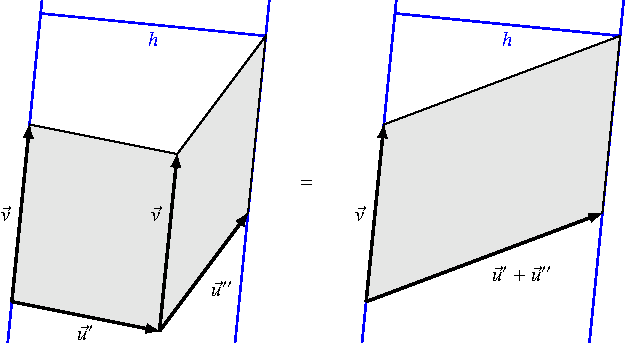
\includegraphics{5/images/flaeche.pdf}
\end{center}
\caption{Addition von Flächeninhalten von Parallelogrammen.
Beide Flächen haben die gleiche Grundseite $|\vec{v}|$ und die gleiche
Höhe $h$, also ist der graue Flächeninhalt beider Figuren gleich.
Daraus lässt sich ableiten, dass der orientierte Flächeninhalt linear
ist in jedem Argument.
\label{image-flaeche-addition}}
\end{figure}
Zwei Vektoren $\vec u$ und $\vec v$ spannen in der Ebene ein Parallelogramm
auf.
Gesucht ist der Flächeninhalt des Parallelogramms.
Statt dafür eine
Formel abzuleiten, untersuchen wir zunächst die Eigenschaften dieses
Flächeninhaltes in der Hoffnung, dass wir bereits ein Objekt mit den
gleichen Eigenschaften kennen.

Wir bezeichnen den Flächeninhalt des von $\vec u$ und $\vec v$ aufgespannten
Parallelogramms mit $A(\vec u,\vec v)$.
Der Flächeninhalt im landläufigen
Sinne ist natürlich immer positiv, es stellt sich jedoch als
zweckmässig heraus, wenn wir den Flächeninhalt hier mit einem
Vorzeichen versehen.
Und zwar soll $A(\vec u,\vec v)$ positiv sein, wenn
sich $\vec u$ mit einer Drehung von weniger als $180^\circ$ in den Vektor
$\vec v$ drehen lässt.
Wir nennen $A(\vec u, \vec v)$ den orientierten
Flächeninhalt.

Die Funktion $A(\vec u,\vec v)$ hat folgende Eigenschaften
\begin{itemize}
\item $A$ ändert das Vorzeichen bei Vertauschung der beiden Vektoren.
\item $A$ ist linear im ersten Argument:
\begin{align*}
A(\vec u'+\vec u'',\vec v)&=A(\vec u',\vec v)+A(\vec v'',\vec u)
\\
A(\lambda \vec u,\vec v)&=\lambda A(\vec u,\vec v)
\end{align*}
\item Der Flächeninhalt eines Einheitsquadrates ist $A(\vec e_1,\vec e_2)=1$.
\end{itemize}
Die beiden Eigenschaften zusammen ergeben, dass $A$ auch linear im
zweiten Argument ist.
Im Kapitel~2 haben wir gelernt, dass es nur eine
Funktion mit diesen Eigenschaften gibt, nämlich die Determinante:
\begin{satz}
Der orientierte Flächeninhalt des von den Vektoren $\vec u$ und $\vec v$
aufgespannten Parallelogramms ist
\[
A(\vec u,\vec v)=\left|\;\begin{matrix}u_1&v_1\\u_2&v_2\end{matrix}\;\right|
=u_1v_2-u_2v_1
.
\]
\end{satz}
\begin{satz}
Der Flächeninhalt eines Dreiecks mit den Ecken $(x_1,y_1)$, $(x_2,y_2)$ und
$(x_3,y_3)$ ist
\[
F=
\frac12\left|\;
\begin{matrix}
x_1-x_3&x_2-x_3\\
y_1-y_3&y_2-y_3\\
\end{matrix}
\;\right|
\]
\end{satz}

\begin{beispiel}
Man berechne den Flächeninhalt des Dreiecks mit den Ecken
$A=(1,6)$, $B=(7,5)$ und $C=(5,3)$.

\smallskip

{\parindent 0pt Die Kantenvektoren} des Dreiecks $ABC$ sind
\[
\overrightarrow{AB}=\begin{pmatrix}6\\-1\end{pmatrix}
,\qquad
\overrightarrow{AC}=\begin{pmatrix}4\\-3\end{pmatrix}
\]
und der Flächeninhalt
\[
F=\frac12\left|\;\begin{matrix}
   6&  4\\
  -1& -3
\end{matrix}\;\right|=
-7
.
\]
Der Flächeninhalt ist also $7$.
\end{beispiel}

\subsection{Volumen eines Parallelepipeds}
\begin{figure}
\begin{center}
%\includegraphics{images/d-2}
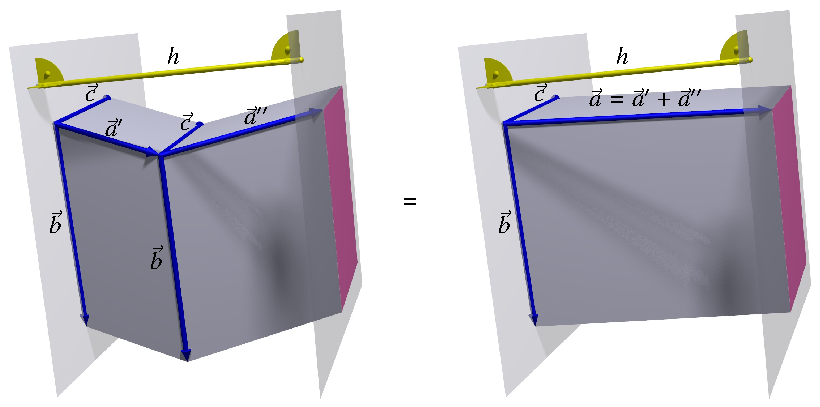
\includegraphics{5/images/volumen.pdf}
\end{center}
\caption{Addition der Volumina von Parallelepipeds.
Da die beiden Körper die gleiche Höhe und die gleiche (pinke) Grundfläche
haben, haben Sie auch das gleiche Volumen.
Daraus kann man ablesen, dass das orientierte Volumen linear ist.
\label{image-volumina}}
\end{figure}
Ganz ähnlich kann man das Volumen eines Parallelepipeds in drei Dimensionen
berechnen, welches von drei Vektoren $\vec a$, $\vec b$ und $\vec c$
aufgespannt wird.
Auch hier stellt es sich als nützlich heraus,
das Volumen mit einem Vorzeichen zu versehen:
\begin{definition}
Das orientierte Volumen
$V(\vec a,\vec b,\vec c)$
eines Parallelepipeds aufgespannt von den drei
Vektoren
$\vec a$, $\vec b$ und $\vec c$ ist positiv, wenn die drei Vektoren
eine ``rechtshändiges System'' bilden, also gegeneinander orientiert
sind wie die ersten drei Finger der rechten Hand, andernfalls ist
$V(\vec a,\vec b,\vec c)$ negativ.
\end{definition}
Dieses orientierte Volumen hat die folgenden Eigenschaften:
\begin{enumerate}
\item Vertauscht man zwei der drei Vektoren, ändert das Volumen das Vorzeichen.
\item $V(\vec a,\vec b,\vec c)$ ist linear im ersten Argument, wie man
der Abbildung~\ref{image-volumina} entnehmen kann:
\begin{align*}
V(\lambda\vec a,\vec b,\vec c)
&=
\lambda V(\vec a,\vec b,\vec c)
\\
V(\vec a'+\vec a'',\vec b,\vec c)
&=
V(\vec a',\vec b,\vec c)
+
V(\vec a'',\vec b,\vec c)
\end{align*}
\item Das orientierte Volumen des Einheitswürfels ist
$V(\vec e_1,\vec e_2,\vec e_3)=1$.
\end{enumerate}
Aus den ersten beiden Eigenschaften können wir folgern, dass das orientierte
Volumen auch in allen anderen Argumenten linear ist.
Und wie im vorangegangenen Abschnitt schliessen wir,
dass $V(\vec a,\vec b,\vec c)$ die Determinante ist:
\begin{satz}
Das orientierte Volumen $V(\vec a,\vec b,\vec c)$ eines von den Vektoren
$\vec a$, $\vec b$ und $\vec c$ aufgespannten Parallepipeds  ist
\[
V(\vec a,\vec b,\vec c)=\left|\;\begin{matrix}
a_1&b_1&c_1\\
a_2&b_2&c_2\\
a_3&b_3&c_3\\
\end{matrix}\;\right|.
\]
\end{satz}
\begin{figure}
\centering
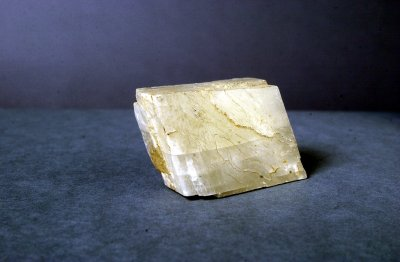
\includegraphics[width=0.7\hsize]{graphics/calcite.jpg}
\caption{Ein Kalzit- oder Kalkspat-Kristall hat die Form eines Parallelepipeds.
Minerale, die sich gut spalten lassen, werden in der Geologie als Spate
bezeichnet, die Spaltprodukte sind angenäherte Parallelepipeds.
\label{skript:orientierung:calcite}}
\end{figure}
Das Parallelepiped wird auch als {\em Spat} bezeichnet.
In der Geologie werden gut spaltbare Minerale als Spate bezeichnet, zum
Beispiel Feldspat oder Kalkspat (Abbildung~\ref{skript:orientierung:calcite}.)
Durch Spaltung gewonnene Kristalle dieser Minerale sind gute Approximationen
von Parallelepipeds.
Das Volumen $V(\vec{a},\vec{b},\vec{c})$ des von $\vec{a}$, $\vec{b}$ und
$\vec{c}$ aufgespannten Parallelepipeds heisst daher auch das Spatvolumen.

\begin{beispiel}
Man finde alle Parallelepipeds mit folgenden Eigenschaften:
\begin{compactenum}
\item Zwei Kanten sind $\vec a=\overrightarrow{OA}$ und $\vec b=\overrightarrow{OB}$
mit $A=(4,1,3)$ und $B=(5,1,2)$.
\item Die dritte Kante ist $\overrightarrow{OC}$, wobei $C$ auf der
Ebene durch $O$ mit der Normalen
\[
\vec n=\begin{pmatrix}1\\1\\1\end{pmatrix}
\]
liegt.
\item Zwei Kanten stehen senkrecht aufeinander.
\item Das Volumen ist $8$.
\end{compactenum}

\smallskip

{\parindent 0pt Wir suchen einen Vektor}
\[
\vec c=\begin{pmatrix}x\\y\\z\end{pmatrix},
\]
der die Bedingungen der Aufgabe erfüllt.
Zunächst muss $\vec c$ auf $\vec n$ senkrecht stehen,
also $\vec c\cdot\vec n=0$ oder
\[
x+y+z=0.
\]
Da $\vec a\cdot\vec b=20+1+6=27\ne 0$ stehen $\vec a$ und $\vec b$
nicht senkrecht, es ist also der gesuchte Vektor $\vec c$ der auf den bereits
bekannten Kanten senkrecht stehen muss.
Wir versuchen es zunächst
mit $\vec a$, weitere Lösungen ergeben sich, wenn man stattdessen $\vec b$
verwendet.
Dies liefert die Bedingung $\vec a\cdot\vec c=0$ oder
\[
4x+y+3z=0
\]
Das Volumen kann mit der Determinante berechnet werden:
\[
V=\left|\;
\begin{matrix}
4&5&x\\
1&1&y\\
3&2&z
\end{matrix}
\;\right|=
4z+15y+2x-3x-8y-5z=-x+7y-z=\pm8.
\]
Jetzt kann der Vektor $\vec c$ mit dem Gauss-Algorithmus bestimmt werden
\begin{align*}
\begin{tabular}{|>{$}c<{$}>{$}c<{$}>{$}c<{$}|>{$}c<{$}|}
\hline
1%
\begin{picture}(0,0)
\color{red}\put(-3,4){\circle{12}}
\end{picture}%
&1&1&0\\
-1&7&-1&\pm8\\
4%
\begin{picture}(0,0)%
\color{blue}\drawline(-12,-2)(-12,24)(4,24)(4,-2)
\end{picture}%
&1&3&0\\
\hline
\end{tabular}
&
\rightarrow
\begin{tabular}{|>{$}c<{$}>{$}c<{$}>{$}c<{$}|>{$}c<{$}|}
\hline
1&1&1&0\\
0&8%
\begin{picture}(0,0)
\color{red}\put(-3,4){\circle{12}}
\end{picture}%
&0&\pm8\\
0&-3%
\begin{picture}(0,0)%
\color{blue}\drawline(-15,-2)(-15,10)(1,10)(1,-2)
\end{picture}%
&-1&0\\
\hline
\end{tabular}
\rightarrow
\begin{tabular}{|>{$}c<{$}>{$}c<{$}>{$}c<{$}|>{$}c<{$}|}
\hline
1&1&1&0\\
0&1&0%
\begin{picture}(0,0)%
\color{blue}\drawline(-8,24)(-8,-2)(2,-2)(2,24)
\end{picture}%
&\pm1\\
0&0&-1%
\begin{picture}(0,0)
\color{red}\put(-7,4){\circle{15}}
\end{picture}%
&\pm3\\
\hline
\end{tabular}
\\
&
\rightarrow
\begin{tabular}{|>{$}c<{$}>{$}c<{$}>{$}c<{$}|>{$}c<{$}|}
\hline
1&1%
\begin{picture}(0,0)%
\color{blue}\drawline(-8,10)(-8,-2)(2,-2)(2,10)
\end{picture}%
&0&\pm3\\
0&1&0&\pm1\\
0&0&1&\mp3\\
\hline
\end{tabular}
\rightarrow
\begin{tabular}{|>{$}c<{$}>{$}c<{$}>{$}c<{$}|>{$}c<{$}|}
\hline
1&0&0&\pm 2\\
0&1&0&\pm1\\
0&0&1&\mp3\\
\hline
\end{tabular}
\end{align*}
Es folgt $C=(\pm 2,\pm1,\mp3)$.
Zwei weitere Lösungen findet
man auf die gleiche Weise, indem man statt der Bedingung $\vec a\cdot\vec c=0$
verlangt, dass $\vec b\cdot\vec c=0$, man findet dann
\begin{align*}
\begin{tabular}{|>{$}c<{$}>{$}c<{$}>{$}c<{$}|>{$}c<{$}|}
\hline
1%
\begin{picture}(0,0)
\color{red}\put(-3,4){\circle{12}}
\end{picture}%
&1&1&0\\
-1&7&-1&\pm8\\
5%
\begin{picture}(0,0)%
\color{blue}\drawline(-12,-2)(-12,24)(4,24)(4,-2)
\end{picture}%
&1&2&0\\
\hline
\end{tabular}
&
\rightarrow
\begin{tabular}{|>{$}c<{$}>{$}c<{$}>{$}c<{$}|>{$}c<{$}|}
\hline
1&1&1&0\\
0&8%
\begin{picture}(0,0)
\color{red}\put(-3,4){\circle{12}}
\end{picture}%
&0&\pm8\\
0&-4%
\begin{picture}(0,0)%
\color{blue}\drawline(-15,-2)(-15,10)(1,10)(1,-2)
\end{picture}%
&-3&0\\
\hline
\end{tabular}
\rightarrow
\begin{tabular}{|>{$}c<{$}>{$}c<{$}>{$}c<{$}|>{$}c<{$}|}
\hline
1&1&1&0\\
0&1&0%
\begin{picture}(0,0)
\color{blue}\drawline(-8,24)(-8,-2)(2,-2)(2,24)
\end{picture}%
&\pm1\\
0&0&-3%
\begin{picture}(0,0)
\color{red}\put(-7,4){\circle{15}}
\end{picture}%
&\pm4\\
\hline
\end{tabular}
\\
&
\rightarrow
\begin{tabular}{|>{$}c<{$}>{$}c<{$}>{$}c<{$}|>{$}c<{$}|}
\hline
1&1%
\begin{picture}(0,0)
\color{blue}\drawline(-8,10)(-8,-2)(2,-2)(2,10)
\end{picture}%
&0&\pm\frac43\\
0&1&0&\pm1\\
0&0&1&\mp\frac43\\
\hline
\end{tabular}
\rightarrow
\begin{tabular}{|>{$}c<{$}>{$}c<{$}>{$}c<{$}|>{$}c<{$}|}
\hline
1&0&0&\pm\frac13\\
0&1&0&\pm1\\
0&0&1&\mp\frac43\\
\hline
\end{tabular}
\end{align*}
also
$C=(\pm\frac13,\pm1,\mp\frac43)$.
\end{beispiel}


%
% vektorprodukt.tex
%
% (c) 2018 Prof Dr Andreas Müller, Hochschule Rapperswil
%

\section{Vektorprodukt}
Das orientierte Volumn in drei Dimensionen ermöglicht die Konstruktion 
des Vektorproduktes.
Mit ihm wird die Aufgabe, einen Vektor senkrecht auf zwei gegebenen
Richtungen zu finden, besonders einfach lösbar.
Es ist aber auch nützlich für eine Reihe von Formeln zur Bestimmung
des Abstandes zwischen Punkt und Gerade oder zwischen windschiefen
Geraden im Raum.

\rhead{Vektorprodukt}
\subsection{Definition des Vektorproduktes}
Wir schreiben das Spatvolumen nach der Sarrusschen Regel aus:
\begin{align*}
V(\vec a,\vec b,\vec c)&=\det(\vec a,\vec b,\vec c)\\
&=
a_1b_2c_3+b_1c_2a_3+c_1a_2b_3
-a_3b_2c_1-b_3c_2a_1-c_3a_2b_1\\
&=
(a_2b_3-a_3b_2)c_1+(a_3b_1-a_1b_3)c_2+(a_1b_2-a_2b_1)c_3
\\
&=
\begin{pmatrix}
a_2b_3-a_3b_2\\
a_3b_1-a_1b_3\\
a_1b_2-a_2b_1
\end{pmatrix}
\cdot
\begin{pmatrix}
c_1\\c_2\\c_3
\end{pmatrix}
\end{align*}
Es gibt also einen Vektor $\vec a\times\vec b$, der die Berechnung
des Spatvolumens mit einem Skalarprodukt erlaubt:
\begin{definition}
Der Vektor
\[
\vec a\times\vec b= \begin{pmatrix}
a_2b_3-a_3b_2\\
a_3b_1-a_1b_3\\
a_1b_2-a_2b_1
\end{pmatrix}
\]
heisst das Vektorprodukt von $\vec a$ und $\vec b$.
Die Komponenten $p_i$
des Vektorproduktes $\vec p=\vec a\times \vec b$ sind
\[
p_1
=
\left|\;\begin{matrix}
a_2&b_2\\a_3&b_3
\end{matrix}\;\right|\\
,\qquad p_2=
\left|\;\begin{matrix}
a_3&b_3\\a_1&b_1
\end{matrix}\;\right|\\
,\qquad p_3=
\left|\;\begin{matrix}
a_1&b_2\\a_2&b_1
\end{matrix}\;\right|.
\]
\end{definition}
\begin{figure}
\centering
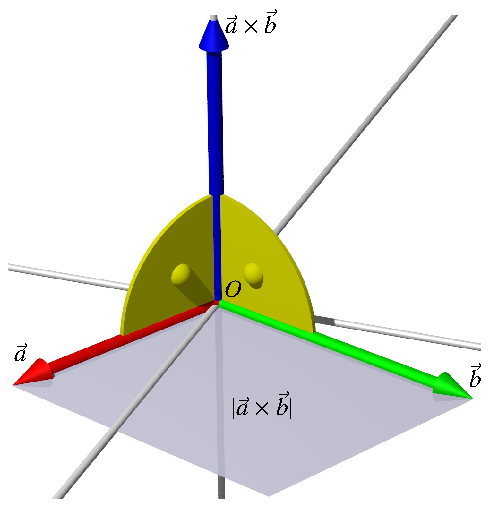
\includegraphics{5/images/vektorprodukt.pdf}
\caption{Das Vektorprodukt der Vektoren $\vec{a}$ und $\vec{b}$ ist ein Vektor
senkrecht auf $\vec{a}$ und $\vec{b}$ mit einer Länge, die dem 
Flächeninhalt des aufgespannten Parallelogramms entspricht und derart,
dass $\vec{a}$, $\vec{b}$ und $\vec{a}\times\vec{b}$ ein Rechtssystem
bilden.
\label{skript:vektorprodukt}}
\end{figure}
Das Vektorprodukt hat die folgenden Eigenschaften (siehe auch
Abbildung~\ref{skript:vektorprodukt}).
\begin{satz}
Sind $\vec a$ und $\vec b$ zwei dreidimensionale Vektoren, dann gilt
\begin{itemize}
\item $\vec a\times\vec b$ steht senkrecht auf $\vec a$ und $\vec b$.
\item $|\vec a\times\vec b|$ ist der Flächeninhalt des von
$\vec a$ und $\vec b$ aufgespannten Parallelogrammes im Raum
\item Ist $\alpha$ der Winkel zwischen $\vec a$ und $\vec b$, dann
ist
\[
|\vec a\times\vec b|=|\vec a|\,|\vec b|\sin \alpha.
\]
\end{itemize}
\end{satz}
\begin{proof}[Beweis]
Sei $\vec c$ ein Vektor in der von $\vec a$ und $\vec b$ aufgespannten
Ebene.
In diesem Fall degeneriert das Parallelepiped, es hat Volumen $0$,
also $V(\vec a,\vec b,\vec c)= 0$.
Da also
\[
V(\vec a,\vec b,\vec c)=(\vec a\times \vec b)\cdot \vec c=0,
\]
steht $\vec c$ senkrecht auf $\vec a\times\vec b$.
Da dies für jeden
Vektor $\vec c$ in der von $\vec a$ und $\vec b$ aufgespannten Ebene
gilt, steht $\vec a\times\vec b$ senkrecht auf dieser Ebene, und insbesondere
auf $\vec a$ und $\vec b$.
Dies beweist die Aussage a).

Sei $\vec n$ der Normalenvektor mit Länge $1$ auf der von $\vec a$ und
$\vec b$ aufgespannten Ebene.
Das Volumen $V(\vec a,\vec b,\vec n)$ ist
dasjenige eines geraden Prismas mit dem von $\vec a$ und $\vec b$
aufgespannten Prisma mit Höhe $1$, also gleich gross wie der
Flächeninhalt des von $\vec a$ und $\vec b$ aufgespannten Parallelogramms.
Andererseits ist
\[
V(\vec a,\vec b,\vec n)=(\vec a\times\vec b)\cdot \vec n
\]
die Projektion des Vektors $\vec a\times\vec b$ auf $\vec n$.
Die beiden
Vektoren haben aber die gleiche Richtung, weil sie beide senkrecht stehen
auf der von $\vec a$ und $\vec b$ aufgespannten Ebene.
Also ist die Projektion
gerade die Länge des Vektors, also ist
$|\vec a\times\vec b|$ der Flächeninhalt des Parallelogramms.

Die Höhe des von $\vec a$ und $\vec b$ aufgespannten Parallelogramms
ist $|\vec b|\sin \alpha$, der Flächeninhalt also
$|\vec a\times\vec b|=|\vec a|\,|\vec b|\sin\alpha.$
\end{proof}

\begin{beispiel}
Man bestimme das Vektorprodukt von
\[
\vec a=\begin{pmatrix}1\\2\\3\end{pmatrix}
\quad\text{und}\quad
\vec b=\begin{pmatrix}8\\5\\13\end{pmatrix}.
\]

\smallskip
{\parindent 0pt Wir verwenden direkt die Definition}
\[
\vec a\times \vec b=
\begin{pmatrix}1\\2\\3\end{pmatrix}
\times
\begin{pmatrix}8\\5\\13\end{pmatrix}
=
\begin{pmatrix}
2\cdot 13-3\cdot 5\\
3\cdot 8-1\cdot 13\\
1\cdot 5-2\cdot 8
\end{pmatrix}
=
\begin{pmatrix}
11\\
11\\
-11
\end{pmatrix}.
\]
\end{beispiel}

\subsection{Normale}
Das Vektorprodukt erlaubt uns jetzt auf einfache Weise die Normale einer
Ebene zu finden.
Sei
\[
\vec r=\vec p+t\vec u+s\vec v
\]
die Parameterdarstellung einer Ebene, dann ist
\[
\vec n=\vec u\times\vec v
\]
eine Normale, also ist
\[
(\vec r-\vec p)\cdot (\vec u\times\vec v)=0
\]
die implizite Form der Ebenengleichung.

\begin{beispiel}
Man finde die Normale der Ebene mit der Gleichung (\ref{beispielebene}).

\smallskip
{\parindent 0pt Die Normale haben wir schon einmal mit Hilfe der Gleichungen
(\ref{gleichungen-fuer-normale}) berechnet, jetzt kann dies
mit Hilfe des vereinfacht werden:}
\begin{equation}
\vec n = \vec u\times \vec v=
\begin{pmatrix}2\\2\\-2\end{pmatrix}
\times
\begin{pmatrix}3\\-3\\-1\end{pmatrix}
=
\begin{pmatrix}
2\cdot(-1)-(-2)\cdot(-3)\\
(-2)\cdot 3-2\cdot (-1)\\
2\cdot(-3)-2\cdot 3
\end{pmatrix}
=
\begin{pmatrix}
-8\\
-4\\
-12
\end{pmatrix}
=-4\begin{pmatrix}2\\1\\3\end{pmatrix}.
\label{beispielvektorprodukt}
\end{equation}
also ein Vielfaches des mit den Gleichungen (\ref{gleichungen-fuer-normale})
gefundenen Normale.
Damit wird die Ebenengleichung
\begin{align*}
0=
\begin{pmatrix} -8\\ -4\\ -12 \end{pmatrix}\cdot
\left(
\begin{pmatrix}x\\y\\z\end{pmatrix}
-
\begin{pmatrix}1\\2\\1 \end{pmatrix}
\right)
&=
-8x-4y-12z+
28
\\
\Rightarrow
2x+y+3z&=7.
\end{align*}
\end{beispiel}

\subsection{Weitere Anwendungen}

\subsubsection{Zwischenwinkel}
Für den Zwischenwinkel zweier Vektoren gilt
\[
\sin\alpha=\frac{|\vec a\times\vec b|}{|\vec a|\cdot|\vec b|}.
\]
\begin{beispiel}
Berechne den Zwischenwinkel der Richtungsvektoren der Ebenengleichung
\ref{beispielebene}.

\smallskip

{\parindent 0pt Das Vektorprodukt der beiden Vektoren wurde
in (\ref{beispielvektorprodukt}) schon
berechnet.} Die Länge der Vektoren ist
\[
|\vec u|=\sqrt{4+4+4}=2\sqrt{3}
,
\quad
|\vec v|=\sqrt{9+9+1}=\sqrt{19}.
\]
Die Zwischenwinkelformel liefert jetzt
\begin{align*}
\sin\alpha&=\frac{|\vec u\times \vec v|}{|\vec u|\cdot |\vec v|}
=\frac{\sqrt{64+16+144}}{\sqrt{12\cdot 19}}
=\frac{\sqrt{224}}{\sqrt{228}}=0.98246\\
\alpha&=79.252^\circ.
\end{align*}
\end{beispiel}

\subsubsection{Abstand Punkt--Gerade}
\begin{figure}
\begin{center}
%\includegraphics{images/d-3}
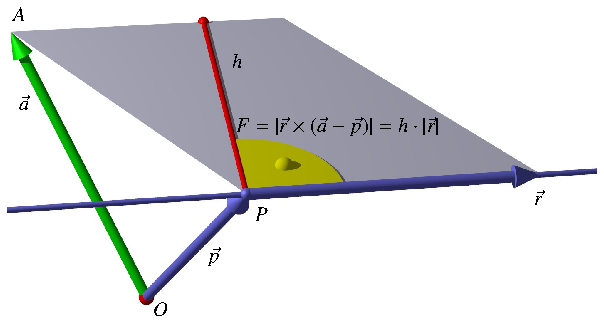
\includegraphics{5/images/abstand.pdf}
\end{center}
\caption{Abstand Punkt--Gerade mit dem Vektorprodukt\label{punkt-gerade}}
\end{figure}
Es ist der Abstand eines Punktes mit Ortsvektor $\vec a$ von der
Geraden durch den Punkt mit Ortsvektor $\vec p$ und Richtungsvektor $\vec r$,
also mit der Parameterdarstellung
\[
\vec q=\vec p+t\vec r
\]
zu bestimmen.
Der gesuchte Abstand $d$ ist die Höhe des Parallelogramms,
welches von $\vec a-\vec p$
und $\vec r$ aufgespannt wird, wobei $\vec r$ als Grundseite zu betrachten ist.
Der Flächeninhalt $A$ des Parallelogramms kann mit dem Vektorprodukt
berechnet werden:
\begin{align*}
A&=|(\vec a-\vec p)\times\vec r|\\
d&=\frac{|(\vec a-\vec p)\times\vec r|}{|\vec r|}.
\end{align*}
\subsubsection{Abstand zweier windschiefer Geraden}
\begin{figure}
\begin{center}
%\includegraphics{images/d-4}
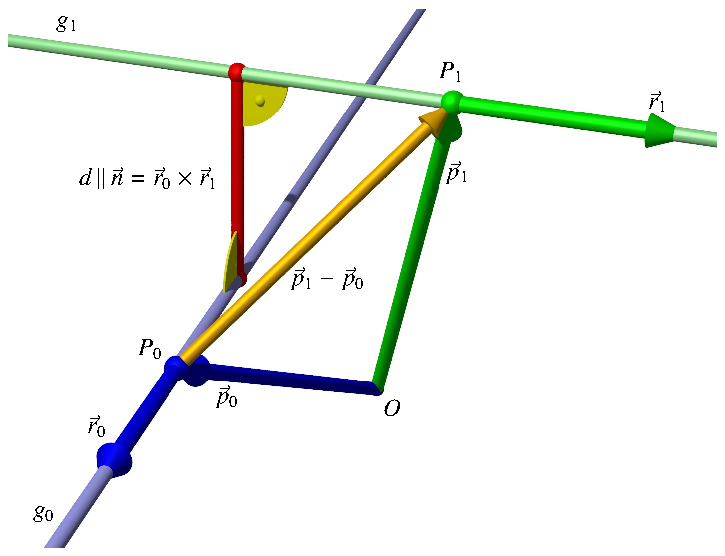
\includegraphics{5/images/windschief.pdf}
\end{center}
\caption{Abstand windschiefer Geraden: der minimale Abstand (rot) ist
parallel zur Normalen auf beide Geraden $g_0$ und $g_1$ also parallel
zum Vektorprodukt $\vec{r_0}\times\vec{r}_1$.
\label{windschief}}
\end{figure}
Zwei nicht parallele Geraden $g_0$ und $g_1$ im Raum,
die sich nicht schneiden, heissen
{\em windschief}.
\index{windschief}
Sie haben
einen kürzesten Abstand $d$, der auf beiden Geraden senkrecht steht.
Sind
\begin{align*}
g_0:
\vec p&=\vec p_0+t\vec r_0\\
g_1:
\vec p&=\vec p_1+t\vec r_1
\end{align*}
Parameterdarstellungen der Geraden, dann ist die Richtung des kürzesten
Abstandes die Richtung des Vektorproduktes $\vec n = \vec r_0\times\vec r_1$.
Ein Vektor zwischen zwei beliebigen Punkten auf den beiden Geraden,
zum Beispiel zwischen $P_0$ und $P_1$, also der Vektor $\vec p_1-\vec p_0$,
wird als Projektion auf die Richtung des kürzesten Abstandes immer die
Länge dieses kürzesten Abstandes haben.
Die Projektion kann mit dem
Skalarprodukt berechnet werden, der kürzeste Abstand $d$ ist
\[
d=(\vec p_1-\vec p_0)\cdot\frac{\vec r_0\times\vec r_1}{|\vec r_0\times\vec r_1|}.
\]


%
% abbildungen.tex
%
% (c) 2018 Prof Dr Andreas Müller, Hochschule Rapperswil
% 
\section{Orientierungserhaltende Abbildungen}
\rhead{Orientierungserhaltende Abbildungen}
Wie im Falle des Skalarproduktes bilden die Abbildungen, die den Flächeninhalt,
das Volumen und/oder die Orientierung erhalten, eine Gruppe.

\subsection{Determinante und Fläche}
Sei $A$ eine Abbildungsmatrix in einem zweidimensionalen Raum.
Die Spalten von $A$ sind die Bilder der Standardbasisvektoren.
Die Determinante von $A$ ist der orientierte Flächeninhalt des Parallelogramms 
aufgespannt von den beiden Spaltenvektoren.
Die von $A$ beschriebene Abbildung macht also aus einem Quadrat mit
orientiertem Flächeninhalt $F$
eine Parallelogramm mit orientierten Flächeninhalt $\det(A)\cdot F$.

Der Flächeninhalt eines Gebietes in der Ebene bleibt unter der Abbildung
$A$ genau dann erhalten, wenn $\det(A)=\pm 1$ gilt.
Falls $\det(A)=-1$ ändert die Orientierung.
Eine Abbildung, die nicht nur den Flächeninhalt, sondern auch die
Orientierung erhält, erfüllt $\det(A)=1$.

Eine Abbildung mit $\det(A)=1$ muss nicht orthogonal sein, wie das Beispiel
\begin{align*}
A
&=
\begin{pmatrix}2&3\\1&2\end{pmatrix}
\qquad\Rightarrow\qquad
\det(A) = 2\cdot 2-3\cdot 1 =1
\\
A^tA
&=
\begin{pmatrix}2&1\\3&2\end{pmatrix}
\begin{pmatrix}2&3\\1&2\end{pmatrix}
=
\begin{pmatrix}
5&7\\
7&13
\end{pmatrix}
\ne
\begin{pmatrix}
1&0\\
0&1
\end{pmatrix}.
\end{align*}
Ausserdem müsste eine orthogonale Matrix Spaltenvektoren der Länge $1$ haben,
während die Spalten von $A$ ganz offensichtlich länger als $1$ sind.

\subsection{Determinante und Volumen}
Aus dem gleichen Argument wie beim Flächeninhalt folgt, dass eine
Abbildungsmatrix $A$ in einem dreidimensionalen Raum einen Körper mit
Volumen $V$ auf einen Körper mit Volumen $\det(A)\cdot V$.
Eine Abbildung $A$ erhält das Volumen, wenn $\det(A)=\pm 1$,
die Orientierung bleibt ebenfalls erhalten, wenn $\det(A)=1$.

\subsection{Spezielle lineare und orthogonale Gruppe}
Die orientientierungserhaltenden Abbildungen bilden die Teilmenge
\[
\operatorname{SL}_n(\mathbb R)
=
\{
A\in M_n(\mathbb R)
\;|\;
\det(A) = 1
\}.
\]
Für $A,B\in\operatorname{SL}_n(\mathbb R)$ lässt die
Produktformel
\[
\det(AB)=\det(A)\det(B) = 1
\]
die Schlussfolgerung zu, dass auch $AB\in\operatorname{SL}_n(\mathbb R)$.
Die Menge $\operatorname{SL}_n(\mathbb R)$ ist daher eine Gruppe, sie
heisst die {\em spezielle lineare Gruppe}.

Abbildungen $A$, die das Skalarprodukt erhalten, sind in $\operatorname{O}(n)$ und erfüllen
\[
A^tA=E
\quad\Rightarrow\quad
1
=
\det(E)
=
\det(A^tA)=\det(A^t)\det(A)=\det(A)^2
\quad\Rightarrow\quad
\det(A) = \pm 1.
\]
Die Abbildungen, die sowohl das Skalarprodukt als auch die Orientierung
erhalten, zeichnen sich also dadurch aus, dass sie sowohl in
$\operatorname{O}(n)$ als auch in $\operatorname{SL}_n(\mathbb R)$ sein, wir nennen diese
Gruppe
\[
\operatorname{SO}(n) 
=
\operatorname{O}(n) \cap \operatorname{SL}_n(\mathbb R)
=
\{
A\in M_n(\mathbb R)\;|\; A^tA=E\wedge \det(A) = 1
\}
\]
die spezielle orthogonale Gruppe.
Dies sind die Bewegungen, die den Nullpunkt unverändert lassen,
Längen und Winkel erhalten und die Orientierung nicht ändern.
Dies sind genau die Drehmatrizen.
Die Determinante ist also das in Abschnitt~\ref{subsection:orthogonale gruppe}
angekündigte Kriterium, mit welchem wir Drehmatrizen von Matrizen
unterscheiden können, die eine Spiegelungskomponente enhalten.

Die Differenz $\operatorname{O}(n) \setminus \operatorname{SO}(n)$
besteht aus Matrizen, die zwar das Skalarprodukt erhalten, aber die
Orientierung umkehren.
Ist $S_x$ die Spiegelung an der Ebene senkrecht zur $x$-Achse und ist
$A\in \operatorname{O}(n) \setminus \operatorname{SO}(n)$, dann ist
\[
\det(S_xA)= \det(S_x)\det(A) = (-1)\cdot(-1)=1
\qquad\Rightarrow\qquad
S_xA\in\operatorname{SO}(n).
\]
Dies bedeutet, dass die Multiplikation mit $S_x$ eine bijektive Abbildung
\[
\operatorname{SO}(n) \to \operatorname{O}(n)\setminus\operatorname{SO}(n)
:
A\mapsto S_xA
\]
definiert.
Die Gruppe $\operatorname{O}(n)$ besteht also aus zwei gleichartig gebauten
Teilmengen, $\operatorname{SO}(n)$  und
$\operatorname{O}(n)\setminus\operatorname{SO}(n)$.




